\documentclass{standalone}
\usepackage{config}
\usetikzlibrary{calc, shadings}

\begin{document}
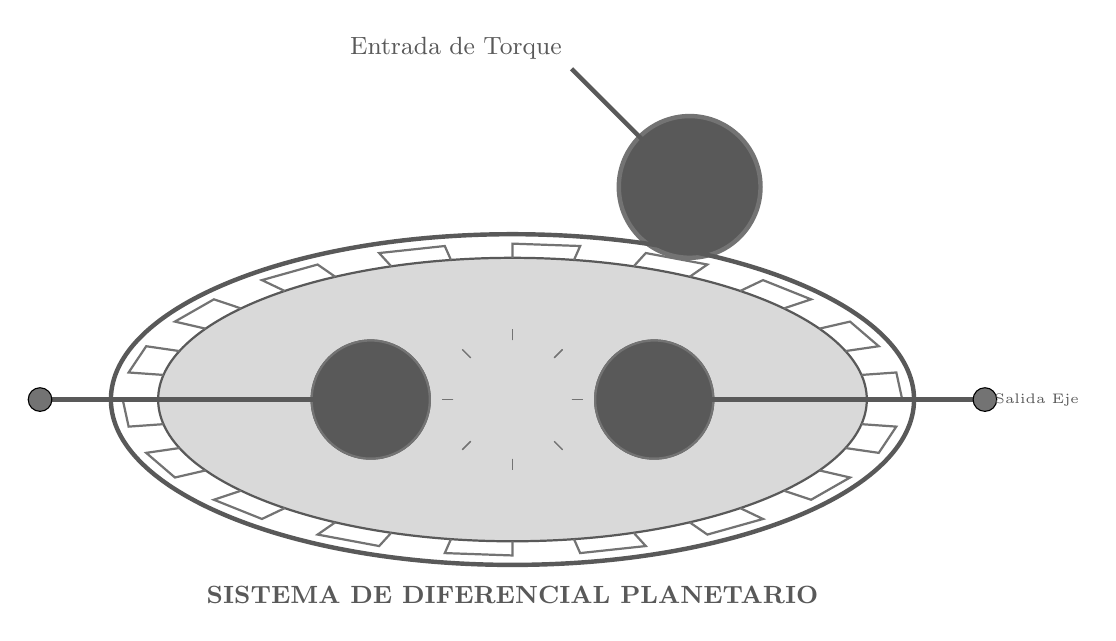
\begin{tikzpicture}[scale=1.5, >=stealth]
    % --- Paleta de Colores Técnicos ---
    \colorlet{steel}{gray!70!black}
    \colorlet{steelbright}{gray!30}
    \colorlet{steeldark}{gray!90!black}

    % --- Coordenadas Base ---
    \coordinate (O) at (0,0);

    % --- Corona (Crown Gear) con Perspectiva ---
    % Sombreado de fondo para volumen
    \fill[steelbright] (O) ellipse (3cm and 1.2cm);
    \draw[steel, thick] (O) ellipse (3cm and 1.2cm);
    
    % Dientes de la corona (Trazado paramétrico)
    \foreach \a in {0,20,...,340} {
        \coordinate (P1) at (\a:3cm);
        \coordinate (P2) at (\a+10:3cm);
        % Proyección a elipse (x, y*0.4)
        \pgfmathsetmacro{\xone}{3*cos(\a)}
        \pgfmathsetmacro{\yone}{1.2*sin(\a)}
        \pgfmathsetmacro{\xtwo}{3*cos(\a+10)}
        \pgfmathsetmacro{\ytwo}{1.2*sin(\a+10)}
        \draw[steeldark, thick] (\xone, \yone) -- (\xone*1.1, \yone*1.1) -- (\xtwo*1.1, \ytwo*1.1) -- (\xtwo, \ytwo);
    }

    % --- Piñón de Ataque (Pinion) ---
    % Posicionado tangencialmente con ajuste de perspectiva
    \coordinate (P) at (1.5, 1.8);
    \draw[fill=steelbright, steel, thick] (P) circle (0.6cm);
    \draw[steeldark, ultra thick] (P) circle (0.6cm);
    % Eje del piñón con degradado
    \draw[steel, ultra thick] ($(P) + (-1, 1)$) -- (P);
    \node[above left, font=\small, steel] at ($(P) + (-1, 1)$) {Entrada de Torque};

    % --- Sistema de Satélites ---
    % Carcasa del diferencial (Housing)
    \draw[steel, ultra thick] (O) ellipse (3.4cm and 1.4cm);
    
    % Satélite 1 (Izquierda)
    \coordinate (S1) at (-1.2, 0);
    \draw[fill=steelbright, steel, thick] (S1) circle (0.5cm);
    \draw[steeldark, thick] (S1) circle (0.5cm);
    % Dientes internos del satélite
    \foreach \a in {0,45,...,315} {
        \draw[steeldark] (\a:0.5cm) -- (\a:0.6cm);
    }

    % Satélite 2 (Derecha)
    \coordinate (S2) at (1.2, 0);
    \draw[fill=steelbright, steel, thick] (S2) circle (0.5cm);
    \draw[steeldark, thick] (S2) circle (0.5cm);
    \foreach \a in {0,45,...,315} {
        \draw[steeldark] (\a:0.5cm) -- (\a:0.6cm);
    }

    % --- Ejes de Salida (Axles) ---
    \draw[steel, ultra thick] (-4,0) -- (S1);
    \draw[steel, ultra thick] (S2) -- (4,0);
    
    % Puntos de apoyo de los ejes
    \draw[fill=steeldark] (-4,0) circle (0.1cm);
    \draw[fill=steeldark] (4,0) circle (0.1cm);

    % --- Etiquetas Técnicas Finales ---
    \node[below, font=\small\bfseries, steel] at (0, -1.5) {SISTEMA DE DIFERENCIAL PLANETARIO};
    \node[below, font=\tiny, steel] at (S1) {Satélite L};
    \node[below, font=\tiny, steel] at (S2) {Satélite R};
    \node[right, font=\tiny, steel] at (4,0) {Salida Eje};

\end{tikzpicture}
\end{document}